\documentclass{article}
\usepackage[spanish]{babel}
\usepackage[utf8]{inputenc}
\usepackage{graphicx}
\usepackage{listings}             % Incluye el paquete listings
\usepackage[T1]{fontenc}
\usepackage{color}
\usepackage{subcaption}
\usepackage{caption}
%\usepackage[backend=bibtex]{biblatex}
%\addbibresource{MiBiblio.bib}
\usepackage{hyperref} %para las refrencias
    \hypersetup{breaklinks=true,colorlinks=true,
        linkcolor=black,citecolor=black,urlcolor=black}
\usepackage{natbib}
\usepackage{xcolor}
\definecolor{miverde}{rgb}{0,0.6,0}
\definecolor{migris}{rgb}{0.5,0.5,0.5}
\definecolor{mimalva}{rgb}{0.58,0,0.82}
\definecolor{gray97}{gray}{.97}
\definecolor{gray75}{gray}{.75}
\definecolor{gray45}{gray}{.45}


\lstset{ %
  backgroundcolor=\color{gray97},   % Indica el color de fondo; necesita que se añada \usepackage{color} o \usepackage{xcolor}
  basicstyle=\footnotesize,        % Fija el tamaño del tipo de letra utilizado para el código
  breakatwhitespace=false,         % Activarlo para que los saltos automáticos solo se apliquen en los espacios en blanco
  breaklines=true,                 % Activa el salto de línea automático
  captionpos=b,                    % Establece la posición de la leyenda del cuadro de código
  commentstyle=\color{miverde},    % Estilo de los comentarios
  deletekeywords={...},            % Si se quiere eliminar palabras clave del lenguaje
  escapeinside={\%*}{*)},          % Si quieres incorporar LaTeX dentro del propio código
  extendedchars=true,              % Permite utilizar caracteres extendidos no-ASCII; solo funciona para codificaciones de 8-bits; para UTF-8 no funciona. En xelatex necesita estar a true para que funcione.
  %frame=single,	                   % Añade un marco al código
  keepspaces=true,                 % Mantiene los espacios en el texto. Es útil para mantener la indentación del código(puede necesitar columns=flexible).
  keywordstyle=\color{blue},       % estilo de las palabras clave
  language=Pascal,                 % El lenguaje del código
  otherkeywords={*,...},           % Si se quieren añadir otras palabras clave al lenguaje
  numbers=left,                    % Posición de los números de línea (none, left, right).
  numbersep=5pt,                   % Distancia de los números de línea al código
  numberstyle=\small\color{migris}, % Estilo para los números de línea
  rulecolor=\color{black},         % Si no se activa, el color del marco puede cambiar en los saltos de línea entre textos que sea de otro color, por ejemplo, los comentarios, que están en verde en este ejemplo
  showspaces=true,                % Si se activa, muestra los espacios con guiones bajos; sustituye a 'showstringspaces'
  showstringspaces=false,          % subraya solamente los espacios que estén en una cadena de esto
  showtabs=true,                  % muestra las tabulaciones que existan en cadenas de texto con guión bajo
  stepnumber=2,                    % Muestra solamente los números de línea que corresponden a cada salto. En este caso: 1,3,5,...
  stringstyle=\color{mimalva},     % Estilo de las cadenas de texto
  tabsize=2,	                   % Establece el salto de las tabulaciones a 2 espacios
  %title=\lstname                   % muestra el nombre de los ficheros incluidos al utilizar \lstinputlisting; también se puede utilizar en el parámetro caption
}


\title{Tarea 1}
\author{Johanna Bolanos Zuniga Matricula: 1883900}
\date{} %aqui puede quedar vacio para que no aparezca la fecha o quitar este comando para que la fecha quede automatica

\begin{document}
\maketitle %para crear el titulo

\section{Grafo simple no dirigido acíclico}
De acuerdo a \cite{Ahuja2017}, es un grafo donde los vértices están conectados por una única arista y su flujo es en dos sentidos. Es decir, un vértice sólo se visita si han sido visitados todos sus predecesores. El código para este grafo programado en Python se muestra en el Listing \ref{1} y el ejemplo gráfico en el la Figura \ref{fig:g1}. Este grafo es útil para representar arboles cronológicos.

\captionof{lstlisting}{Código en Python del grafo simple no dirigido acíclico}\label{1}
\lstinputlisting[language=Python]{G1.py} 
%\noindent{Fuente: Elaboración propia basado en \citep{networkx}}


\begin{figure}[htp]
\centering
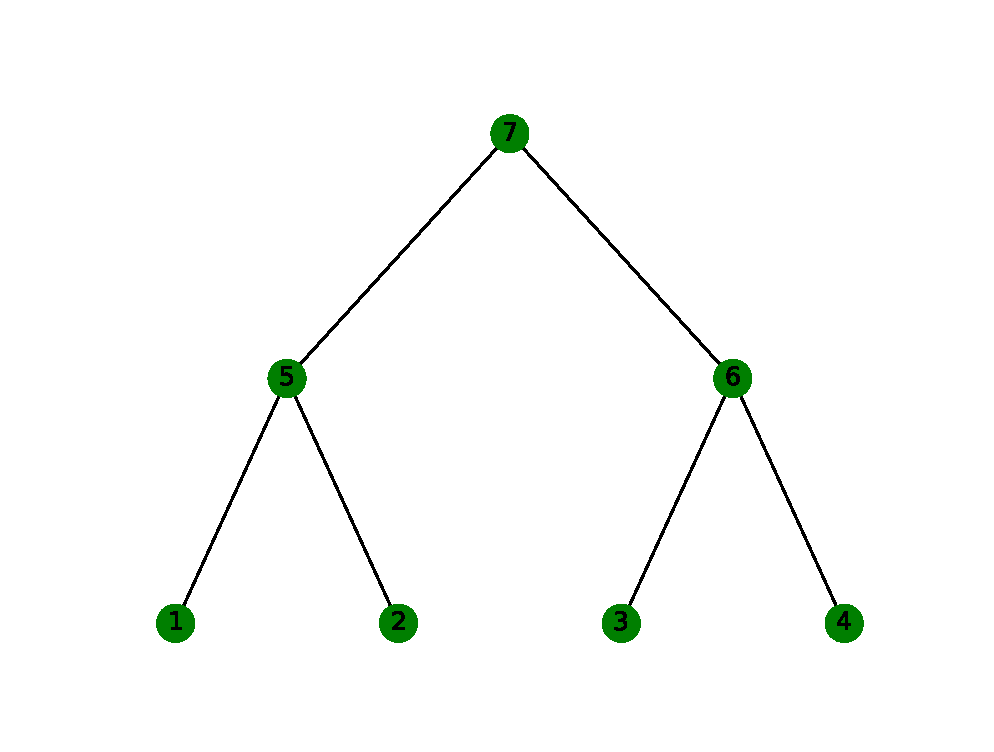
\includegraphics[scale=0.4]{g1.eps}
\caption{Ejemplo del grafo simple no dirigido acíclico}
\label{fig:g1}
\noindent{Fuente: Elaboración propia}
\end{figure}


\section{Grafo simple no dirigido cíclico}
Cuando dos vértices de un grafo están conectados sin direccionamiento por dos aristas diferentes formando un ciclo, es decir, una trayectoria donde se regresa al punto de partida.



\section{Grafo simple no dirigido reflexivo}
Con base a \citet{elisa, park}, es cuando el grafo cuenta con bucles, es decir, no hay trayectoria, coincide el vértice de partida con el de llegada $(v,v)$ y la arista que los une no tiene direccionamiento.


\section{Grafo simple dirigido acíclico}
De acuerdo a \citet{Ahuja2017}, es un grafo donde los vértices están conectados por una única arista y su flujo es en un solo sentido. Es decir, un vértice sólo se visita si han sido visitados todos sus predecesores. Por ejemplo, los pasos a seguir para hacer una tarea especifica.
%Todas las conexiones, representadas con flechas, están identificadas por un único camino simple que no repite vértices. Es decir, un vértice sólo se visita si han sido visitados todos sus predecesores. 



\section{Grafo simple dirigido cíclico}
Cuando dos vertices de un grafo están asociados ordenamente por dos caminos distintos formando un ciclo.


\section{Grafo simple dirigido reflexivo}
De acuerdo a \cite{elisa}, cuando el grafo cuenta con bucles, es decir, no hay trayectoria, coincide el vértice de partida con el de llegada y la arista que lo une es una flecha arqueada (lazo).
%Cuando el grafo cuenta con bucles, es decir, se queda en el mismo vértice y se une por medio de una arista direccionada (tipo felcha).



\section{Multigrafo no dirigido acíclico}
Cuando en un grafo existen varios caminos, no direccionados, para llegar al destino, es decir, cada par de vertice puede tener más de una arista y el punto de partida es diferente al de llegada.


 
\section{Multigrafo no dirigido cíclico}
\subsection{Explicación}
Cuando en un grafo existen varios caminos sin direccionamiento para llegar al destino, es decir, varias trayectorias que regresan al punto de partida. 



\section{Multigrafo no dirigido reflexivo}
Cuando el grafo cuenta con bucles, es decir, no hay trayectoria, coincide el vértice de partida con el de llegada y la arista que lo une es un lazo no dirigido. Pero, además, en una pareja de vértices hay, al menos, dos aristas sin direccionamiento.


\section{Multigrafo dirigido acíclico}
Cuando en un grafo existen varios caminos indicados por flechas para llegar al destino, es decir, en cada par de vértices hay  más de una arista y el punto de partida es diferente al de llegada. Ejemplo, cuando en la fabricación de un producto se pueden hacer tareas simultaneas.




\section{Multigrafo dirigido cíclico}
Cuando en un grafo existen varios caminos para llegar al destino, es decir, varias trayectorias direccionadas que regresan al punto de partida. Ejemplo, el ciclo hidrológico o la representación del VRP (por sus siglas en inglés, \textit{Vehicule Routing Problem}).


\section{Multigrafo dirigido reflexivo}
Cuando el grafo cuenta con bucles, es decir, no hay trayectoria, coincide el vértice de partida con el de llegada y la arista que lo une es una flecha arqueada. Pero, además, en una pareja de vértices hay al menos dos aristas direccionadas.



\bibliographystyle{mighelnat}
\bibliography{MiBiblio}


\end{document}
